% UrbanFix -- IEEE Access manuscript (LaTeX)
% Compile with the official IEEE Access LaTeX template files
% (ieeeaccess.cls, spotcolor.sty, logo.png, notaglinelogo.png, bullet.png)
% in the same folder, e.g. by uploading main.tex, figs/ and photos/ into
% the "IEEE Access LaTeX Template" project on Overleaf.
\documentclass{ieeeaccess}
\usepackage{cite}
\usepackage{amsmath,amssymb,amsfonts}
\usepackage{graphicx}
\usepackage{textcomp}
\usepackage{booktabs}
\usepackage{array}
\usepackage{url}
\usepackage{tikz}

% filled / half / empty markers used in Tables II and III
\definecolor{markink}{HTML}{1F3A5F}
\definecolor{markline}{HTML}{8A94A6}
\newcommand{\yes}{\tikz[baseline=-0.6ex]\fill[markink] (0,0) circle (2.1pt);}
\newcommand{\part}{\tikz[baseline=-0.6ex]{\draw[markink,line width=0.5pt] (0,0) circle (2.1pt);\fill[markink] (0,-2.1pt) arc (-90:90:2.1pt) -- cycle;}}
\newcommand{\no}{\tikz[baseline=-0.6ex]\draw[markline,line width=0.5pt] (0,0) circle (2.1pt);}

\begin{document}
\history{Date of publication xxxx 00, 0000, date of current version xxxx 00, 0000.}
\doi{10.1109/ACCESS.2026.Doi Number}

\title{UrbanFix: A Closed-Loop, AI-Validated Urban Governance Platform with a Public Accountability Registry and Privacy-Preserving Research Data Access}

\author{\uppercase{Parth Pancholi}\authorrefmark{1},
\uppercase{Gaurav Soni}\authorrefmark{1}, \IEEEmembership{(Senior Member, IEEE)},
\uppercase{Kamlesh Chandravanshi}\authorrefmark{1},
\uppercase{Mahendra Sahare}\authorrefmark{2}, and
\uppercase{Jay Prakash Maurya}\authorrefmark{1}}

\address[1]{School of Computing Science and Engineering, VIT Bhopal University, Bhopal, India (e-mail: parth.25bce10443@vitbhopal.ac.in; gaurav.soni@vitbhopal.ac.in; kamlesh.chandravanshi@vitbhopal.ac.in; jpeemaurya@gmail.com)}
\address[2]{School of Computer Science and Engineering, VIT-AP University, Amaravati, India (e-mail: mahendra.sahare@vitap.ac.in)}

\markboth
{P. Pancholi \headeretal: UrbanFix: A Closed-Loop, AI-Validated Urban Governance Platform}
{P. Pancholi \headeretal: UrbanFix: A Closed-Loop, AI-Validated Urban Governance Platform}

\corresp{Corresponding author: Mahendra Sahare (e-mail: mahendra.sahare@vitap.ac.in).}

\begin{abstract}
Most digital grievance systems classify complaint text and track tickets. They rarely check the photo a citizen attaches, their urgency estimates cannot be traced to inputs, and only the administration sees the records. We present UrbanFix, an urban governance platform that follows a complaint from the citizen's photo to a verified, publicly recorded repair and on to research data. Citizens file without an account using an email code. A YOLOv8 model trained for the chosen category localises the defect in each photo, and a weighted questionnaire gives an urgency score anyone can recompute. A seven-stage workflow enforced on the server requires ward-level assignment, photo proof and a receipt before closure. Every complaint is published without personal data, and approved researchers get logged, time-limited access to an anonymised projection. Validation mAP50 is 0.724 for potholes and 0.502 for litter (masks), and 0.908 for open manholes and 0.729 for graffiti (boxes), at 19 to 33 ms per image on a laptop CPU. When the model is unsure, it flags the report for a human reviewer.
\end{abstract}

\begin{keywords}
e-governance, smart cities, civic technology, object detection, YOLOv8, human-in-the-loop AI, open data, privacy-preserving data sharing
\end{keywords}

\titlepgskip=-21pt

\maketitle

\section{Introduction}

\PARstart{I}{n} India, pothole-related road accidents rose from 3,713 in 2020 to 5,432 in 2024, an increase of 46\%, and pothole-related accidents killed 8,963 people between 2018 and 2022 \cite{b1,b2}. The national grievance portal CPGRAMS received between 18.7 and 26.2 lakh grievances a year from 2019 to 2024 \cite{b3,b4}, and in FY 2023--24 State and Union Territory governments, which handle municipal complaints, took 119 days on average to dispose of one, against 16 days for central ministries \cite{b5} (Fig.~\ref{fig:f1}).

Fig.~\ref{fig:f1}(a) shows pothole accidents dipping slightly in 2021, peaking at 5,840 in 2023 and staying above 5,000 in 2024, so the problem grew over the five years. In Fig.~\ref{fig:f1}(b) the light bars are the backlog carried over from the previous year, which fell from 10.7 lakh in 2020 to 3.1 lakh in 2024; the portal now clears most of what it receives. The dark bars are new grievances, and they reached their highest value, 26.2 lakh, in the same year. Faster disposal has not reduced the number of people who need to complain, so this paper looks at what happens to a complaint after it is filed.

\begin{figure}[!t]
\centering
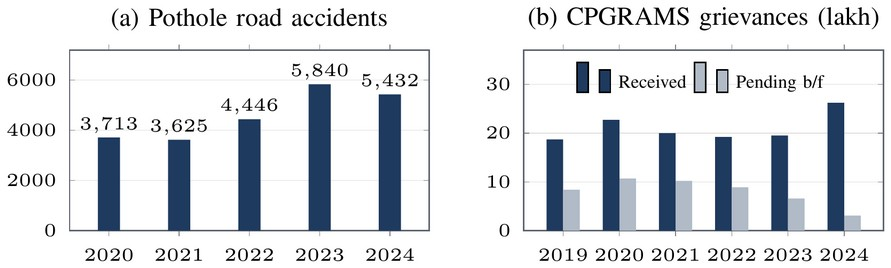
\includegraphics[width=0.89\columnwidth]{figs/fig01.jpg}
\caption{Motivation: (a) pothole-related road accidents in India \cite{b2}; (b) grievances received on CPGRAMS and the backlog brought forward each year \cite{b3,b4}.}
\label{fig:f1}
\end{figure}

Recent systems route complaint text \cite{b6,b7}, predict urgency \cite{b8}, classify waste images \cite{b9} or filter unsafe photos \cite{b10}. None of them checks whether a photo shows the reported defect or lets anyone trace an urgency label back to its inputs, and their records stay with officials or the person who filed. UrbanFix runs each complaint through six steps in one system (Fig.~\ref{fig:f2}). Our contributions are:

\begin{enumerate}
\item A YOLOv8 check \cite{b11} for each category, offered only where a public dataset with localised labels exists.
\item Prioritisation that puts the questionnaire score and the model's evidence in front of a supervisor, who decides; the model cannot reject a report.
\item A workflow modelled as a guarded state machine with ward-level assignment, photo proof and an append-only history.
\item A public registry with identity removed on the server, and a research gateway with scoped, expiring and logged access to pseudonymised records.
\end{enumerate}

Fig.~\ref{fig:f2} reads clockwise from the top. A citizen reports without an account, and the model for the chosen category checks the photo. A supervisor then sets the priority with the questionnaire score $u_Q$ and the model's suggestion $u_{AI}$ side by side. Field staff carry out the work inside the state machine of Eq.~(\ref{eq:e6}) and prove the repair with photos, the citizen receives a PDF receipt, and the closed record feeds the public registry and the research dataset. The centre of the ring is a single complaint record. Every step reads and appends to the same document, so the history the public and researchers see is the one staff produced while working.

\begin{figure}[!t]
\centering
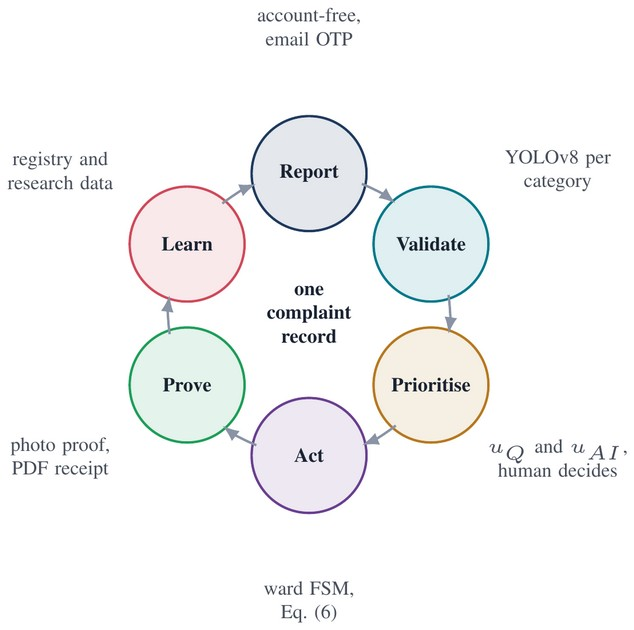
\includegraphics[width=0.63\columnwidth]{figs/fig02.jpg}
\caption{The six steps every complaint passes through in UrbanFix.}
\label{fig:f2}
\end{figure}

\begin{table*}[!t]
\caption{Literature survey}
\label{tab:t1}
\centering
\footnotesize
\setlength{\tabcolsep}{3pt}
\renewcommand{\arraystretch}{1.1}
\begin{tabular}{@{}>{\centering\arraybackslash}p{0.035\textwidth}p{0.18\textwidth}p{0.4\textwidth}p{0.33\textwidth}@{}}
\toprule
S.No. & Authors & Work done & Limitations\\
\midrule
\multicolumn{4}{@{}l}{\textit{A. AI-assisted complaint management}}\\
1 & Chen \textit{et al.} \cite{b20}, 2022 & Treat complaint routing as text classification on real government service records, with automatic label correction that merges highly similar labels. & Complaint text only; evaluated on one partner's records.\\
2 & Javali \textit{et al.} \cite{b21}, 2025 & Infra-Alert: web portal with automatic geolocation, cloud-stored photos, before/after repair photos and PDF reports. & AI verification and prioritisation left as future work; citizens see only their own complaints.\\
3 & Vishwanath \textit{et al.} \cite{b9}, 2025 & ReGenX: Android waste app with geofenced collection alerts, an on-device complaint classifier (90.1\%) and a waste-image classifier (85.2\%). & Waste collection only; needs the app and an account; the image model sorts waste type and does not check the reported problem.\\
4 & Kanagapriya and Kesika \cite{b6}, 2026 & CitiWatch: anonymous reporting with mobile OTP; TF-IDF features and a supervised classifier route text to ten departments with 96.8\% accuracy. & Phone number stays linked to each complaint; no photo evidence; no public registry.\\
5 & Cholke \textit{et al.} \cite{b8}, 2026 & VidyutSaathi: Sentence-BERT multi-task network for severity and resolution time, DBSCAN duplicate clustering and workload-aware assignment, tested on over 20,000 electricity complaints. & Electricity complaints only; urgency is a network output the citizen cannot trace; no public view.\\
6 & Salunkhe \textit{et al.} \cite{b10}, 2026 & CivicMate: photo upload with automatic location, SMS updates and community upvoting; NudeNet screens photos for unsafe content (F1 0.97). & Screening only checks that an image is safe, so a photo of something else still passes; registration required.\\
7 & Katkar \textit{et al.} \cite{b22}, 2026 & CivicX: grievance routing with geospatial heat maps plus ML screening of building plans; 91.4\% classification accuracy against 94.1\% for officers. & Below manual accuracy; transparency limited to officials' dashboards; photos not checked against the complaint.\\
8 & Praveen Kumar \textit{et al.} \cite{b7}, 2026 & Smart City Concern: portal and X posts routed by zero-shot BART (92.8\%), with DistilBERT sentiment for priority, OCR on photos and TF-IDF duplicate linking. & Sentiment stands in for urgency, which the authors note may not reflect real severity; official dashboard only.\\
\multicolumn{4}{@{}l}{\textit{B. Citizen reporting and 311 data}}\\
9 & King and Brown \cite{b23}, 2007 & Evaluated FixMyStreet, an early UK site where residents post local problems and follow them until they are fixed; over 3,000 reports and updates in its first six months. & Council officers reported duplicate reports, difficulty confirming fixes and managing expectations.\\
10 & Goodchild \cite{b24}, 2007 & Introduced volunteered geographic information, with citizens acting as sensors, and examined contributor motives, data accuracy and privacy. & Conceptual review; the accuracy of volunteered data is left as an open question.\\
11 & Clark \textit{et al.} \cite{b12}, 2013 & Tested one year of Boston service requests for race, education and income bias using geospatial analysis and negative binomial regression. & Poorer neighbourhoods used the service less, and Hispanic residents may use it less as requests move online.\\
\bottomrule
\end{tabular}
\end{table*}

\begin{table*}[!t]
\addtocounter{table}{-1}
\caption{Literature survey (continued)}
\centering
\footnotesize
\setlength{\tabcolsep}{3pt}
\renewcommand{\arraystretch}{1.1}
\begin{tabular}{@{}>{\centering\arraybackslash}p{0.035\textwidth}p{0.18\textwidth}p{0.4\textwidth}p{0.33\textwidth}@{}}
\toprule
S.No. & Authors & Work done & Limitations\\
\midrule
12 & Minkoff \cite{b25}, 2016 & Modelled tract-level variation in New York 311 contact volume for goods, graffiti and noise complaints with spatial regression. & Volume reflects the propensity to contact as well as conditions, which makes 311 data hard to use for locating problems.\\
13 & Pak \textit{et al.} \cite{b13}, 2017 & Compared 30,041 FixMyStreet reports from Brussels with socio-demographic statistics and geotagged Twitter data. & Use varied by district, and low-income and ethnically diverse communities were under-represented among those reporting.\\
14 & Wang \textit{et al.} \cite{b26}, 2017 & Showed that the mix of 311 request types in New York, Boston and Chicago acts as a neighbourhood signature that groups areas by socio-economic profile. & Uses aggregate request counts for planning; individual complaints are not handled.\\
15 & Kontokosta and Hong \cite{b14}, 2021 & Linked Kansas City 311 reports with a resident survey, code violations and street assessments to classify neighbourhoods as under- or over-reporting. & Low-income and minority areas reported street issues less despite greater need, so decisions driven by complaint counts can be unfair.\\
\multicolumn{4}{@{}l}{\textit{C. Vision models for civic defects}}\\
16 & Redmon \textit{et al.} \cite{b27}, 2016 & YOLO: one network predicts boxes and classes for the whole image in a single pass, at 45 frames/s (155 for Fast YOLO). & More localisation errors than the strongest detectors of the time.\\
17 & Maeda \textit{et al.} \cite{b28}, 2018 & 9,053 smartphone images from seven Japanese municipalities with 15,435 instances of eight road-damage types; detector run on a GPU server and a smartphone. & Japanese roads only; road damage only.\\
18 & Dhiman and Klette \cite{b29}, 2020 & Reviewed pothole detection and compared two stereo-vision methods with two deep-learning models for the road ahead of a vehicle. & Designed for vehicle cameras; potholes only.\\
19 & Fan \textit{et al.} \cite{b30}, 2020 & Transform a dense disparity map and fit a quadratic road surface to find potholes, at about 98.7\% pixel-level accuracy. & Needs stereo disparity input; potholes only.\\
20 & Arya \textit{et al.} \cite{b31}, 2021 & 26,620 smartphone images from several countries; tested whether a model trained in Japan transfers and proposed generalised models. & Road damage only; detections are not linked to complaint handling.\\
21 & Córdova \textit{et al.} \cite{b32}, 2022 & Compared five detector families on the new PlastOPol set (2,418 images) and TACO; YOLOv5x reached AP50 of 84.9 and 63.3, and YOLOv5s ran on a phone. & All models struggled with small items such as cigarette butts and gave false positives on natural backgrounds.\\
22 & Fogaça \textit{et al.} \cite{b33}, 2023 & Lisbon images classified as illegal graffiti, street art or none (81.4\% accuracy), then illegal graffiti localised (70.3\% IoU). & Weakest on images without graffiti (F1 66\%); one city.\\
\multicolumn{4}{@{}l}{\textit{D. Open data, urban computing and AI in government}}\\
23 & Janssen \textit{et al.} \cite{b34}, 2012 & Used interviews and a workshop to list what open data offers and what holds back its use, and set out five myths about it. & Finds that publishing data is often assumed to bring use and benefit by itself; qualitative study.\\
24 & Zheng \textit{et al.} \cite{b35}, 2014 & Reviewed how city data are collected, stored, combined and analysed, with examples from seven application areas. & Survey of methods; no complaint-handling system is proposed.\\
25 & Wirtz \textit{et al.} \cite{b36}, 2019 & Reviewed the literature to map where governments apply AI (ten areas) and what makes it hard (four groups of challenges). & Conceptual overview without implementation or evaluation.\\
\multicolumn{4}{@{}l}{\textit{E. Human oversight and privacy}}\\
26 & Sweeney \cite{b37}, 2002 & Defined $k$-anonymity, where each released record is indistinguishable from at least $k-1$ others, and examined re-identification attacks. & Releases can still be attacked when the accompanying release policies are not followed.\\
27 & Amershi \textit{et al.} \cite{b38}, 2019 & Proposed 18 guidelines for human-AI interaction and tested them with 49 practitioners on 20 AI products. & General guidelines; the study also found gaps in current knowledge.\\
28 & Wu \textit{et al.} \cite{b39}, 2022 & Surveyed human-in-the-loop machine learning, grouped by where people step in: preparing data, training the model, or designing the whole system. & Survey; identifies open challenges rather than a deployable design.\\
\bottomrule
\end{tabular}
\end{table*}

\section{Related Work}\label{sec:rw}

Table~\ref{tab:t1} groups 28 studies into five strands. Recent complaint platforms (A) route text with 90 to 97\% accuracy, yet none of them checks the photo against the reported defect. Studies of FixMyStreet and 311 data (B) find that who reports, and how often, varies with income and ethnicity \cite{b12,b13,b14}, so complaint counts alone are a biased guide to need. Detectors for road damage, potholes, litter and graffiti (C) are evaluated apart from any complaint workflow. Strands D and E cover open data, AI in government, human oversight and anonymised release. Table~\ref{tab:t2} compares UrbanFix with the seven platforms closest to it. Localised datasets now exist for road damage \cite{b15,b16}, litter \cite{b17}, open manholes \cite{b18} and graffiti \cite{b19}.

\section{System Architecture}\label{sec:arch}

One Expo client serves all six roles, and the server decides which screens a user sees (Fig.~\ref{fig:f3}). Each request passes an Express pipeline that re-checks the account, any pending invitation and research expiry on every call. Intake sends photos to a separate FastAPI service only after returning the tracking ID, so a slow or failed model call cannot affect the filing. Each MongoDB complaint document embeds its status history and AI analysis.

\begin{figure*}[!t]
\centering
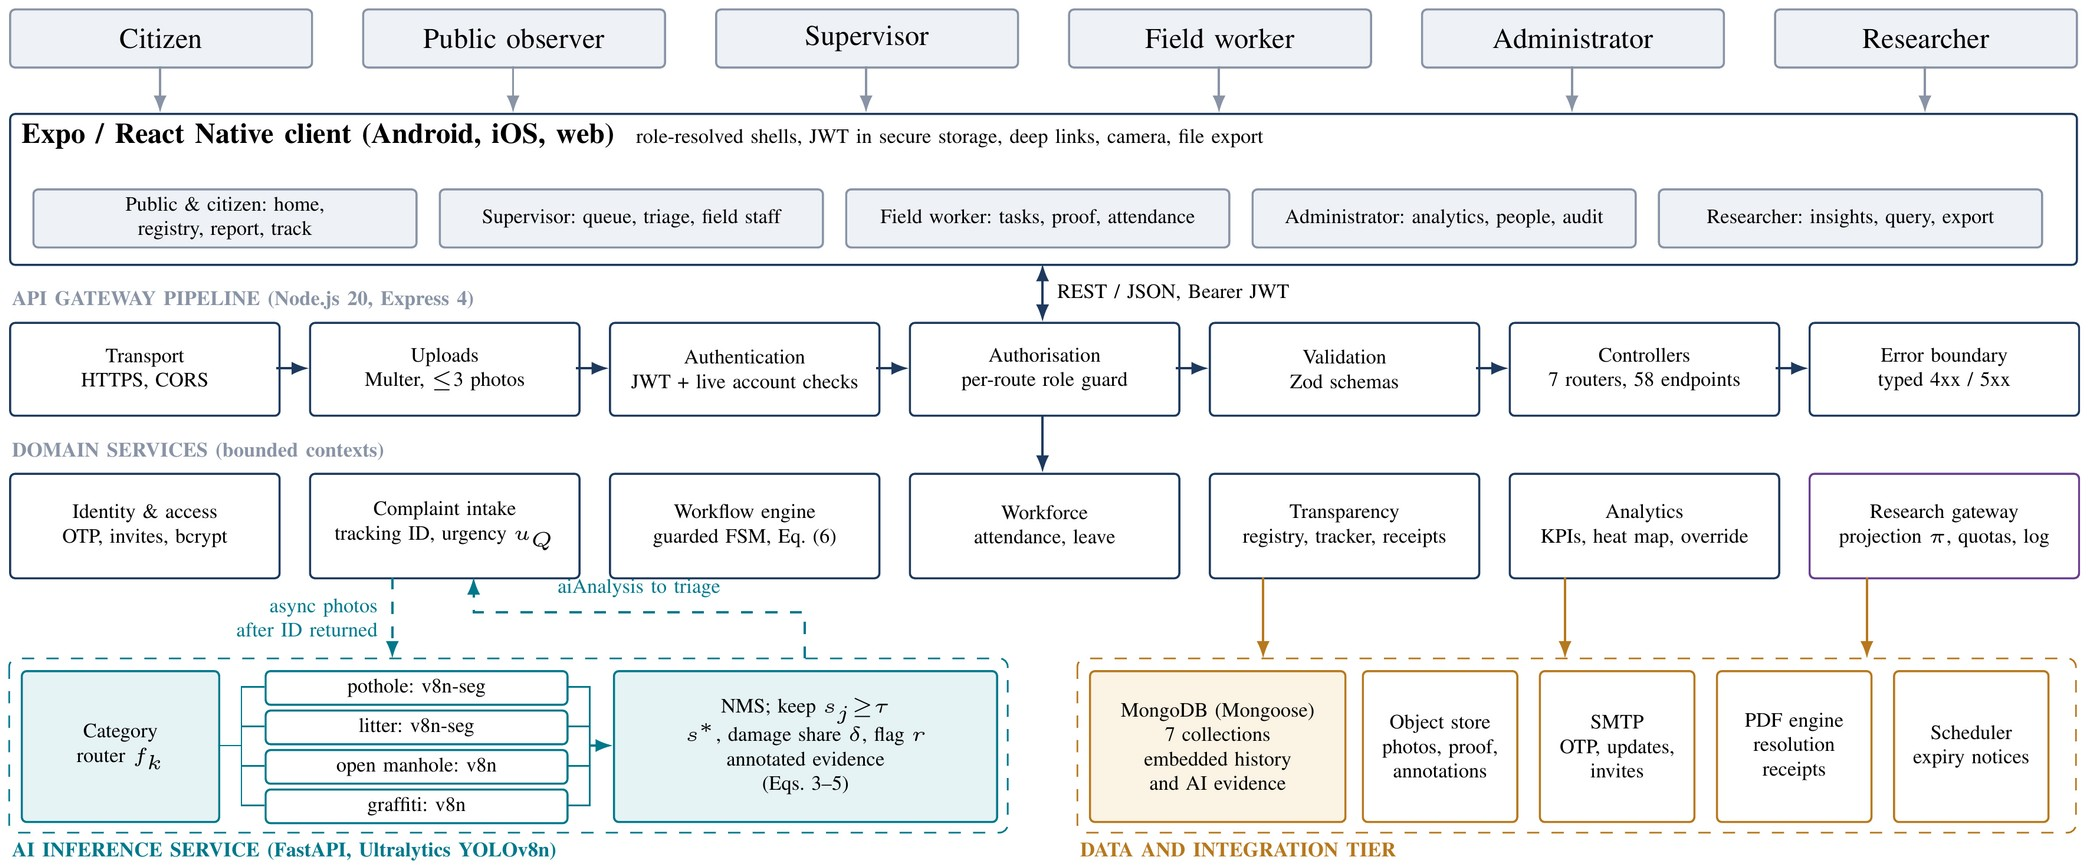
\includegraphics[width=1.00\textwidth]{figs/fig03.jpg}
\caption{Layered architecture of UrbanFix. Solid arrows are synchronous requests. Dashed arrows show the AI call, which is made asynchronously after the tracking ID has been returned. The security and privacy controls of Sections~\ref{sec:wf}--\ref{sec:priv} apply to all layers.}
\label{fig:f3}
\end{figure*}

\begin{table}[!t]
\caption{Capabilities of reviewed systems and UrbanFix (UF)}
\label{tab:t2}
\centering
\footnotesize
\setlength{\tabcolsep}{3.2pt}
\begin{tabular}{@{}l*{7}{c}c@{}}
\toprule
Capability & \cite{b21} & \cite{b6} & \cite{b8} & \cite{b9} & \cite{b10} & \cite{b22} & \cite{b7} & UF\\
\midrule
Account-free filing & \no & \part & \no & \no & \no & \no & \no & \yes\\
Photo evidence & \yes & \no & \part & \yes & \yes & \yes & \part & \yes\\
Photo--defect validation & \no & \no & \part & \no & \no & \no & \no & \yes\\
Urgency scoring & \no & \no & \yes & \no & \no & \yes & \yes & \yes\\
Traceable urgency & \no & \no & \no & \no & \no & \no & \no & \yes\\
Automated routing & \part & \yes & \yes & \part & \yes & \yes & \yes & \part\\
Field proof of repair & \yes & \no & \no & \no & \no & \no & \no & \yes\\
Resolution receipt & \part & \no & \no & \no & \no & \no & \no & \yes\\
Public registry & \no & \no & \no & \no & \part & \no & \no & \yes\\
Open research data & \no & \no & \no & \no & \no & \no & \no & \yes\\
\bottomrule
\multicolumn{9}{@{}l}{\scriptsize \yes~supported \quad \part~partial \quad \no~not supported or not reported}
\end{tabular}
\end{table}

Fig.~\ref{fig:f3} reads from top to bottom. The six actors use the same client, which gives each of them one of five role shells; citizens and the public share one. Every call then passes the seven gateway stages in order, so a request that fails authentication never reaches validation or a controller. Seven domain services sit below the gateway. The research gateway is drawn in purple because it is the only path to bulk data. In the lower left tier, a router sends each photo to one of four YOLOv8n models, and a post-processing step computes the evidence of Eqs.~(\ref{eq:e3})--(\ref{eq:e5}). The lower right tier holds MongoDB and the services for files, email, receipts and scheduled expiry notices. The two dashed arrows are the only asynchronous paths: photos go to the model after the citizen already has a tracking ID, and the result returns as \texttt{aiAnalysis} for triage.

\section{Methodology}\label{sec:method}

\subsection{Category Selection by Dataset Availability}

Let $\mathcal{K}$ be the candidate complaint categories. A category $k$ is offered only if a public dataset $\mathcal{D}_k$ of street-level images with localised labels (boxes or masks), documented provenance and a usable licence exists:

\begin{equation}
\mathcal{C}=\{\,k\in\mathcal{K} : \mathcal{D}_k \text{ is public} \wedge \text{localised} \wedge \text{street-level} \wedge \text{documented} \wedge \text{licensed}\,\}.
\label{eq:e1}
\end{equation}
\noindent Four of ten candidate categories qualify (Fig.~\ref{fig:f4}), and the API rejects the rest.

In Fig.~\ref{fig:f4} each bar is the size of the largest public dataset we found for that category, on a log scale, and the four circles show whether it meets each criterion. Electrical poles have the second largest dataset, 25,426 images, but its labels are only partly localised and its source is undocumented. Water leakage has localised labels, but its images are not street-level and its source is also undocumented. Graffiti has only 1,022 images and meets every criterion, so it is kept. The three smallest candidates have fewer than 1,000 images; road signs and fallen trees also lack a documented source, and the streetlight data has no localised labels. Only the four categories with every circle filled satisfy Eq.~(\ref{eq:e1}).

\subsection{Traceable Questionnaire Urgency}

Each category has five yes/no questions $q_i$ with weights $w_i\in\{1,2\}$ (2 for safety-critical). With answers $y_i\in\{0,1\}$, the urgency score and band are

\begin{equation}
U=\frac{\sum_{i=1}^{5} w_i y_i}{\sum_{i=1}^{5} w_i},\qquad
u_Q=\begin{cases}\text{High}, & U\ge 0.6\\ \text{Medium}, & 0.3\le U<0.6\\ \text{Standard}, & U<0.3.\end{cases}
\label{eq:e2}
\end{equation}
\noindent Dividing by $\sum w_i$ keeps categories with different weights comparable. The citizen sees $u_Q$ while filing, and anyone can recompute it from the stored answers (Fig.~\ref{fig:f5}).

\begin{figure}[!t]
\centering
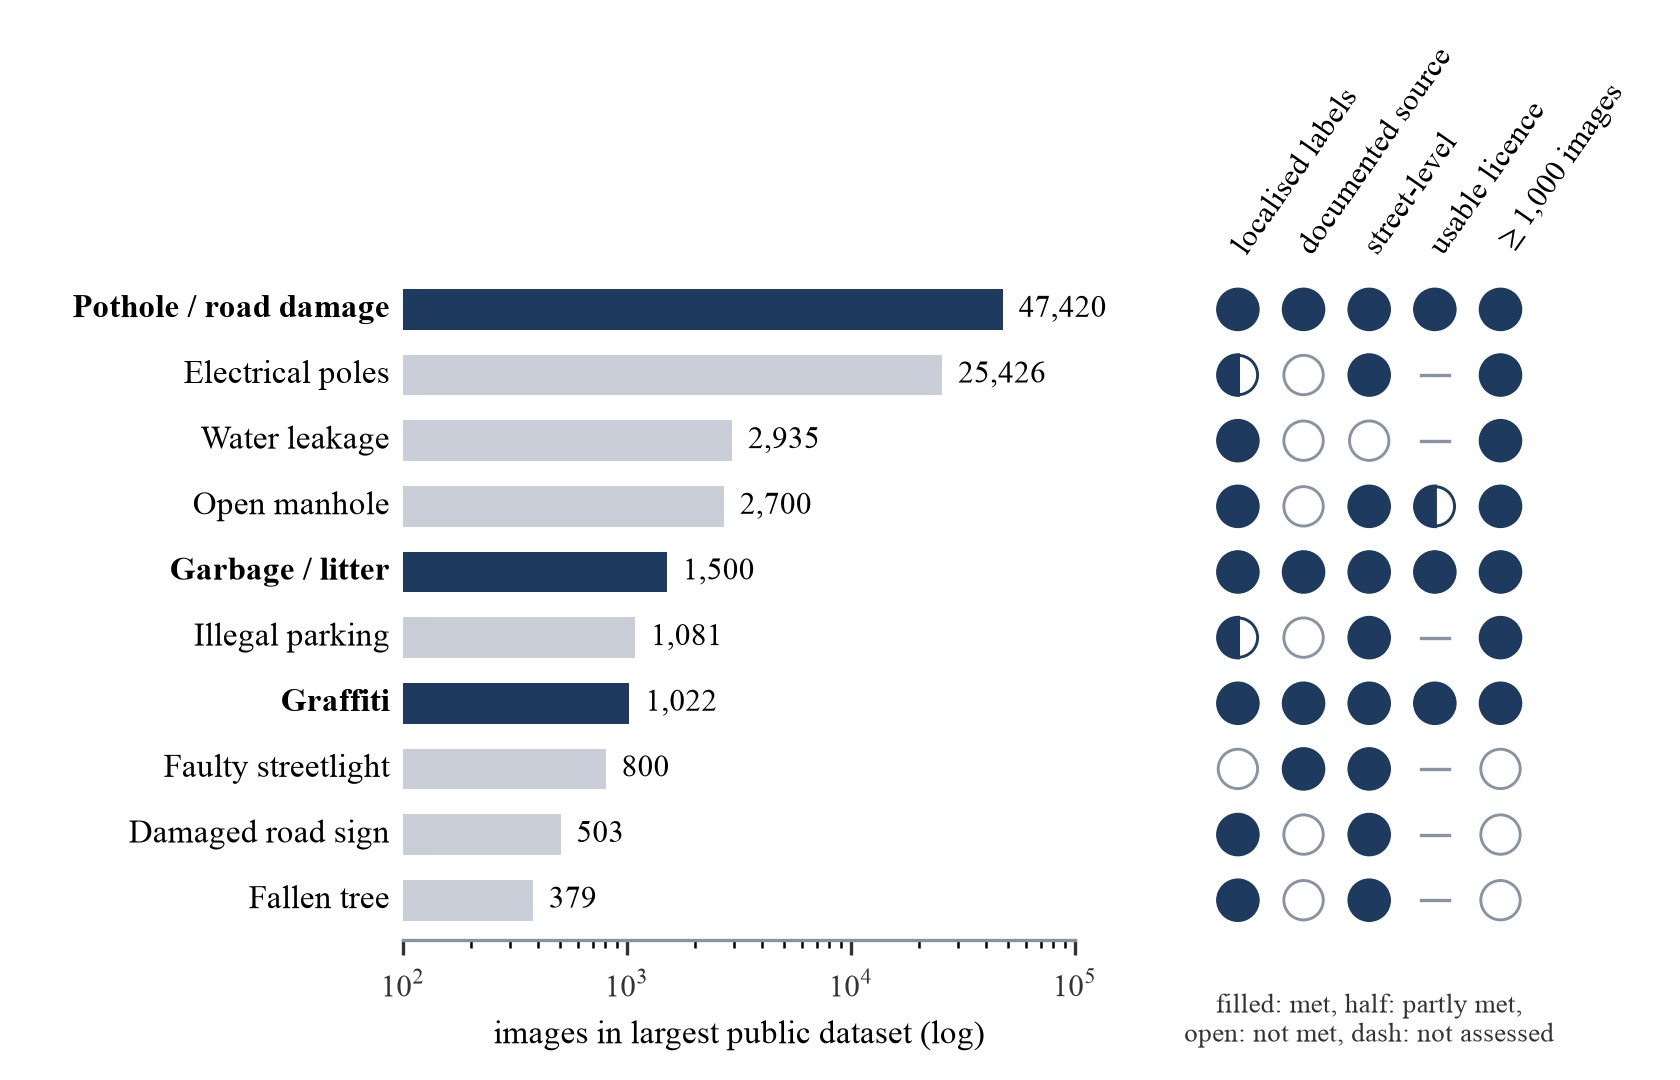
\includegraphics[width=0.96\columnwidth]{figs/fig04.jpg}
\caption{Screening of ten candidate categories against Eq.~(\ref{eq:e1}). Dark bars mark the four categories kept; circles show each criterion met, partly met or not met.}
\label{fig:f4}
\end{figure}

Fig.~\ref{fig:f5} plots every score Eq.~(\ref{eq:e2}) can produce. The pothole and manhole questionnaires mark two questions as safety-critical, so their weights sum to 7 and $U$ moves in steps of 1/7. Litter and graffiti mark one, so the sum is 6 and the steps are 1/6. Both profiles have reachable scores in all three bands, but the same answers can land in different bands. One safety-critical ``yes'' gives a pothole $2/7=0.29$, just short of Medium, while the same answer for litter gives $2/6=0.33$ and reaches Medium. A pothole is rated High only when its ``yes'' answers carry at least 5 of the 7 weight points.

\begin{figure}[!t]
\centering
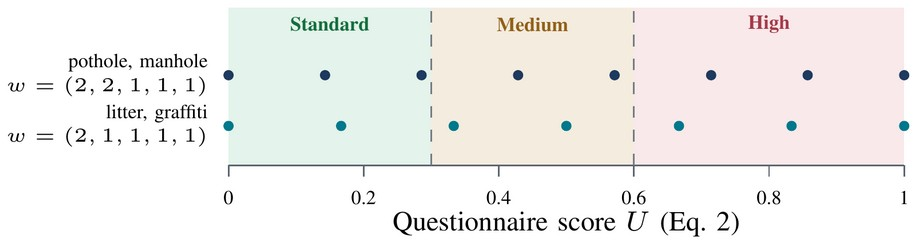
\includegraphics[width=0.91\columnwidth]{figs/fig05.jpg}
\caption{All reachable questionnaire scores for the two weight profiles, with the urgency bands. For a pothole, a single safety-critical ``yes'' scores $2/7=0.29$ and stays in Standard.}
\label{fig:f5}
\end{figure}

\subsection{Per-Category Vision Validation}\label{sec:ai}

For a complaint of category $k$ with photos $x_1,\dots,x_n$ ($n\le3$), the model $f_k$ returns detections $\mathcal{B}_m=f_k(x_m)=\{(b_j,s_j,M_j)\}$ with boxes $b_j$, confidences $s_j$ and, for segmentation models, masks $M_j$. The service keeps detections with $s_j\ge\tau$ ($\tau=0.25$) after non-maximum suppression and computes

\begin{align}
s^{*}&=\max_{m}\max_{j} s_j, \label{eq:e3}\\
\delta&=\max_{m}\frac{\bigl|\bigcup_j M_j^{(m)}\bigr|}{H_m W_m}, \label{eq:e4}\\
r&=\mathbf{1}\left[s^{*}<\tau\right], \label{eq:e5}
\end{align}
\noindent where $\delta$ is the masked share of the image and $r$ is the \texttt{needsReview} flag. The suggested urgency $u_{AI}$ is $u_Q$ raised one band when $\delta>\theta_\delta$. The model never changes a complaint's stage; the supervisor decides with all of this in view (Fig.~\ref{fig:f6}).

Fig.~\ref{fig:f6} shows the order of events. The questionnaire score is computed while the citizen files, and the tracking ID is returned before any inference runs, so the dashed call to the model is the only step that can be slow. The model's detections are reduced to $s^{*}$ and $\delta$ and then tested once. If $s^{*}\ge\tau$, the service suggests $u_{AI}$. If not, it sets $r=1$ and the supervisor works from $u_Q$ alone (the dotted line). Both branches end in the same triage box, so a photo the model could not confirm still reaches a person, with a flag, and is never rejected automatically.

\begin{figure}[!t]
\centering
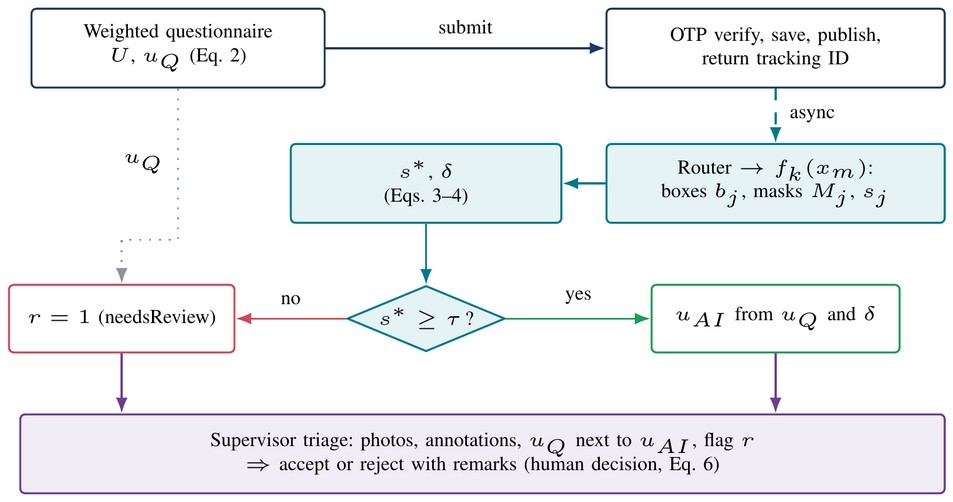
\includegraphics[width=0.95\columnwidth]{figs/fig06.jpg}
\caption{AI validation and prioritisation. The supervisor sees both urgency signals; a low-confidence result sets \texttt{needsReview} and the report stays in the queue.}
\label{fig:f6}
\end{figure}

\subsection{Accountable Workflow}\label{sec:wf}

The workflow is a deterministic finite-state machine $\mathcal{M}=(S,A,\Delta,s_0,F)$ (Fig.~\ref{fig:f8}) with

\begin{align*}
S&=\{\mathrm{sub},\mathrm{acc},\mathrm{asg},\mathrm{wip},\mathrm{prf},\mathrm{cls},\mathrm{rej}\},\\
A&=\{\mathit{accept},\mathit{reject},\mathit{assign},\mathit{start},\mathit{proof},\mathit{close},\mathit{rework}\},
\end{align*}
\noindent start $s_0=\mathrm{sub}$ and terminal set $F=\{\mathrm{cls},\mathrm{rej}\}$. A transition is applied only if its guard holds:

\begin{equation}
\Delta(s,a)\ \text{is defined} \iff s\in\mathcal{S}_a \wedge \rho(\text{actor})\in\mathcal{R}_a \wedge g_a(c),
\label{eq:e6}
\end{equation}
\noindent where $\mathcal{S}_a$ and $\mathcal{R}_a$ are the allowed source stages and roles, and the guard $g_a$ checks remarks ($\ge$10 characters), the ward and leave status of the assignee, and the proof photos. Each transition appends (stage, actor, remarks, $t$) to the history, and \textit{close} emails a PDF receipt. The public sees $\varphi(s)\in\{$Pending, In Progress, Resolved, Rejected$\}$.

Fig.~\ref{fig:f8} shows every path a complaint can take. The main path runs through five transitions from submitted to closed, and Eq.~(\ref{eq:e6}) guards each one. Rejection is possible only from the submitted stage. After acceptance the only terminal stage left is closed, and reaching it requires proof. If the supervisor finds the proof inadequate, the dashed rework arrow returns the task to assigned, and the loop on assigned lets the supervisor hand it to another worker without changing the stage. The fill colours give the public status. A citizen sees In Progress for all four middle stages, so internal handoffs do not appear on the tracker.

\begin{figure*}[!t]
\centering
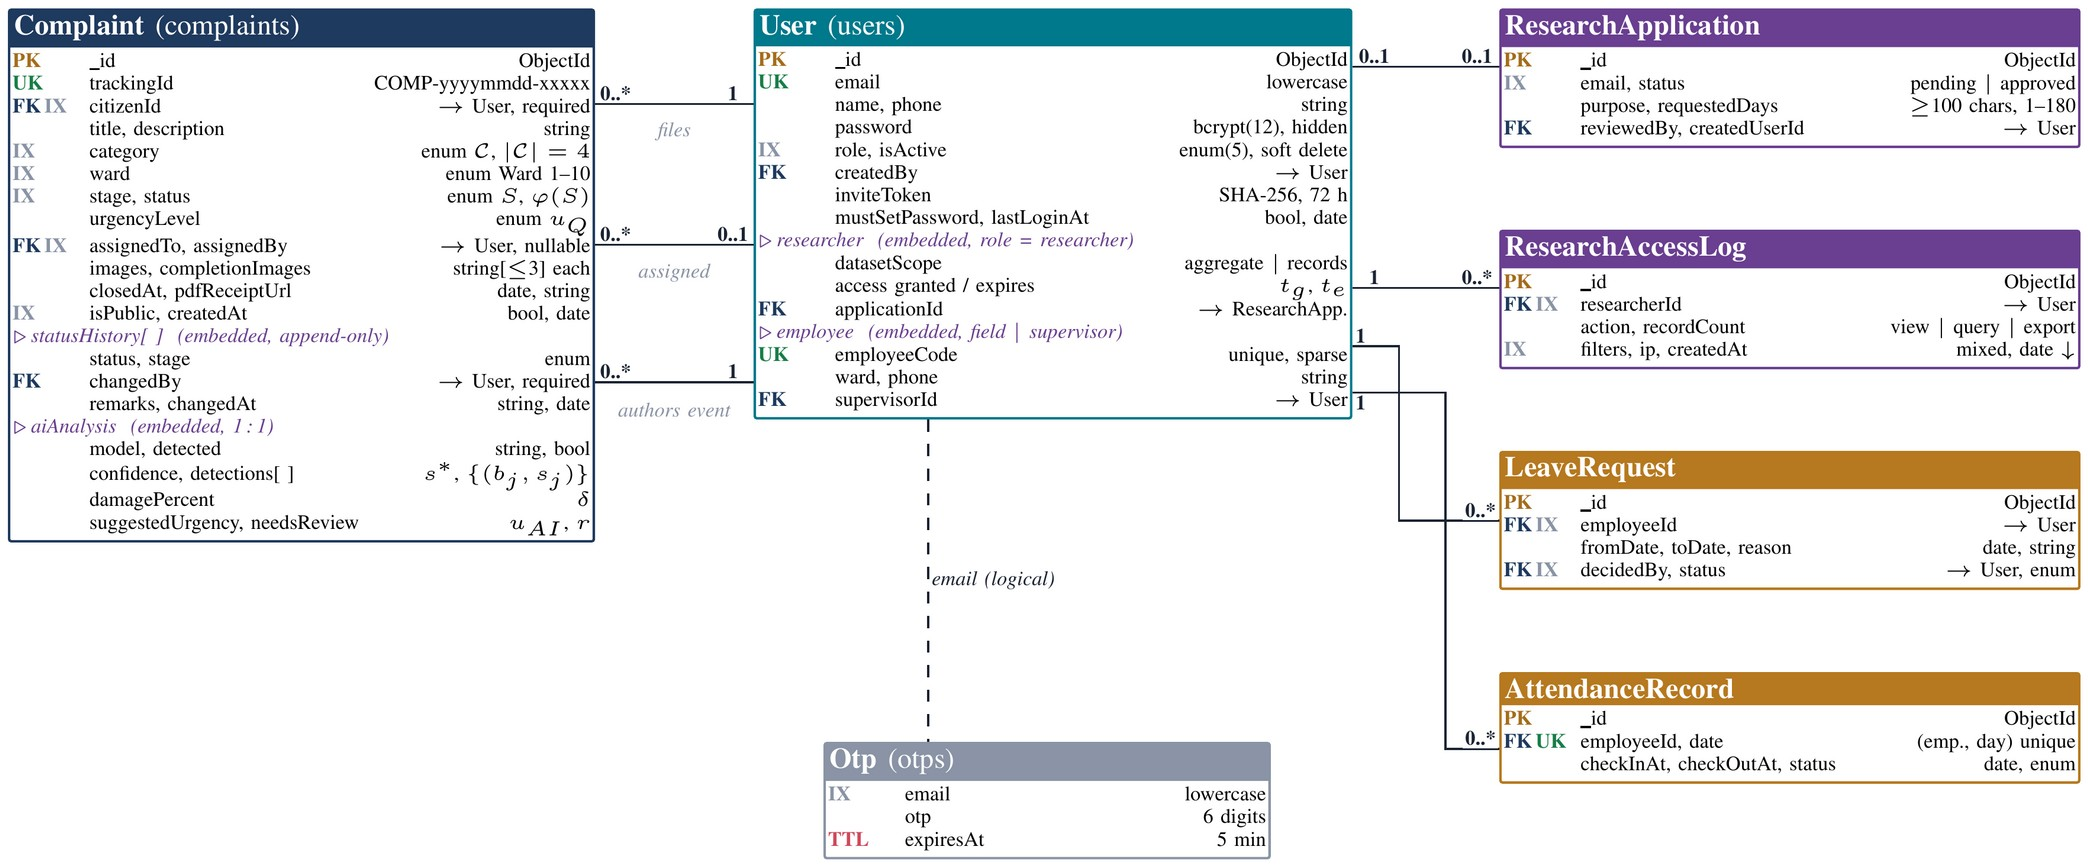
\includegraphics[width=1.00\textwidth]{figs/fig07.jpg}
\caption{Physical data model (MongoDB, Mongoose schemas). PK, FK, UK, IX and TTL mark primary keys, references, unique, secondary and expiry indexes; rows marked $\triangleright$ begin embedded sub-documents. Multiplicities follow UML notation.}
\label{fig:f7}
\end{figure*}

\subsection{Tiered Disclosure and Research Projection}\label{sec:priv}

Each audience gets a fixed server-side projection of the same record (Table~\ref{tab:t3}). Researchers get eight fields

\begin{equation}
\pi(c)=\bigl(h_\kappa(c.\mathit{id}),\,k,\,u_Q,\,\varphi,\,\mathit{ward},\,\lfloor t_f\rfloor_{d},\,\lfloor t_c\rfloor_{d},\,\Delta t\bigr),
\label{eq:e7}
\end{equation}
\begin{equation}
h_\kappa(x)=\mathrm{trunc}_{48}\bigl(\mathrm{HMAC\text{-}SHA256}(\kappa,x)\bigr),\quad \Delta t=\tfrac{t_c-t_f}{86400\,\mathrm{s}},
\label{eq:e8}
\end{equation}
\noindent where $\lfloor\cdot\rfloor_d$ truncates to the day and $\kappa$ is a server secret, so IDs join across exports but cannot be reversed. A request $q$ under scope $\sigma$ and expiry $t_e\le t_g+180$ days is served only if

\begin{equation}
\begin{aligned}
&t_q<t_e\ \wedge\ \bigl(\mathrm{rows}(q)\Rightarrow\sigma=\mathrm{records}\bigr)\\
&\wedge\ n_{\mathrm{exp}}(d)\le5\ \wedge\ |q|\le5000,
\end{aligned}
\label{eq:e9}
\end{equation}
\noindent Fig.~\ref{fig:f9} follows a researcher from application to data. The first three steps happen once. The applicant states a purpose, an administrator sets the scope $\sigma$ and the expiry $t_e$, and the invitation link is stored only as a SHA-256 hash and lapses after 72 hours. The last three steps repeat on every request. The server checks Eq.~(\ref{eq:e9}) and answers 403 or 429 if any part fails. A request that passes receives only the projection $\pi(c)$, and the request is written to the access log.

\begin{figure}[!t]
\centering
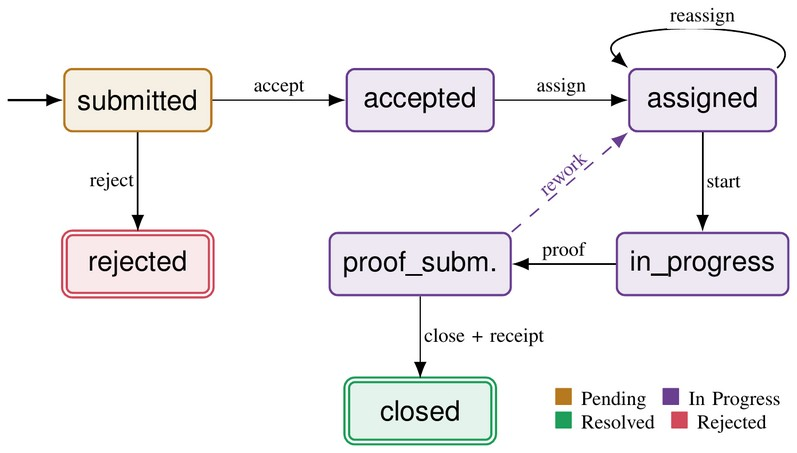
\includegraphics[width=0.79\columnwidth]{figs/fig08.jpg}
\caption{Server-enforced complaint lifecycle (Eq.~\ref{eq:e6}). Fill colour gives the public status $\varphi(s)$; double borders mark terminal stages.}
\label{fig:f8}
\end{figure}

\begin{table}[!t]
\caption{Disclosure of one complaint record by audience}
\label{tab:t3}
\centering
\footnotesize
\setlength{\tabcolsep}{1.9pt}
\begin{tabular}{@{}lcccccc@{}}
\toprule
Attribute & Admin & Staff & Registry & Tracker & Res. rec. & Res. agg.\\
\midrule
Citizen identity & \yes & \no & \no & \no & \no & \no\\
Staff identity & \yes & \yes & \no & \part & \no & \no\\
Record ID & \yes & \yes & \yes & \yes & \part & \no\\
Title, description, photos & \yes & \yes & \yes & \yes & \no & \no\\
Street location & \yes & \yes & \yes & \yes & \part & \no\\
Category, urgency, status & \yes & \yes & \yes & \yes & \yes & \part\\
Timestamps & \yes & \yes & \yes & \yes & \part & \part\\
History with remarks & \yes & \yes & \part & \yes & \no & \no\\
\bottomrule
\multicolumn{7}{@{}l}{\scriptsize \part~transformed: HMAC ID, ward-level, day-level or aggregated.}
\end{tabular}
\end{table}

\begin{figure}[!t]
\centering
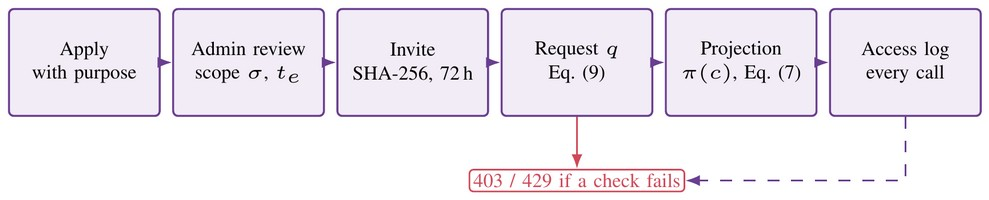
\includegraphics[width=0.99\columnwidth]{figs/fig09.jpg}
\caption{Research access chain. Expiry, scope and quotas are checked on every request, and every request is logged.}
\label{fig:f9}
\end{figure}

\subsection{Data Model}

One User collection holds all five roles, and Complaint embeds its history and AI analysis (Fig.~\ref{fig:f7}). Staff accounts are only ever deactivated, so history entries keep a valid actor.

Every relationship line in Fig.~\ref{fig:f7} ends at User. A complaint points to users in three ways: the citizen who filed it (exactly one), the worker it is assigned to (none or one), and the actor of each history event (one per event). The four collections on the right attach to User in the same way. A user has at most one research application and any number of access-log entries, leave requests and attendance records, and a unique index allows one attendance record per employee per day. Otp is joined by a dashed line because it is matched by email, not by a stored reference, and its TTL index removes each code five minutes after it is issued. Because the history and the AI evidence are embedded, each complaint loads as a single document without a join.

\section{Implementation and Experimental Setup}\label{sec:impl}

The stack is Expo 57, Node.js 20 with Express and Mongoose, and FastAPI with Ultralytics 8.4 \cite{b11}. Each model is fine-tuned from COCO YOLOv8n weights at $640\times640$, batch 16, up to 60 epochs with patience 15, on an Apple M5 laptop (Table~\ref{tab:t4}, Fig.~\ref{fig:f11}); training took 29 to 52 minutes.

We report precision $P=TP/(TP+FP)$, recall $R=TP/(TP+FN)$ and

\begin{equation}
\mathrm{AP}=\int_{0}^{1} p(r)\,dr,
\label{eq:e10}
\end{equation}
\noindent with mAP50 at IoU 0.5 and mAP50--95 averaged over 0.50 to 0.95.

\begin{table}[!t]
\caption{Datasets and models per category}
\label{tab:t4}
\centering
\footnotesize
\setlength{\tabcolsep}{2.2pt}
\begin{tabular}{@{}llccc@{}}
\toprule
Category & Dataset & Labels & Train/val & Model\\
\midrule
Pothole / road damage & Roboflow \cite{b16} & masks & 720/60 & v8n-seg\\
Garbage / litter & TACO \cite{b17} & masks$^{\dagger}$ & 1214/214 & v8n-seg\\
Open manhole & Road Hazards \cite{b18} & boxes & 1123/480 & v8n\\
Graffiti & STORM \cite{b19} & boxes & 813/209 & v8n\\
\bottomrule
\multicolumn{5}{@{}l}{\scriptsize $^{\dagger}$60 TACO classes merged into one; 1,428 of 1,500 images still available.}
\end{tabular}
\end{table}

\section{Results and Discussion}\label{sec:res}

\subsection{Validation Models}

Table~\ref{tab:t5} and Figs.~\ref{fig:f11}--\ref{fig:f14} give the results. Open manholes score highest (box mAP50 0.908), though augmented copies in that dataset may inflate it. Graffiti is precise but misses faint tags (recall 0.604), and litter is hardest (0.502) because TACO's 60 classes were merged into one. These misses are why Eq.~(\ref{eq:e5}) only flags reports. Inference takes 19 to 33 ms per photo on CPU (Table~\ref{tab:t5}), so no GPU server is needed. Fig.~\ref{fig:f10} shows stored outputs and app screens.

\begin{table}[!t]
\caption{Validation results (best checkpoint)}
\label{tab:t5}
\centering
\footnotesize
\setlength{\tabcolsep}{3.4pt}
\begin{tabular}{@{}lccccc@{}}
\toprule
Model (metric set) & $P$ & $R$ & mAP50 & mAP50--95 & CPU ms\\
\midrule
Pothole (mask) & 0.725 & 0.711 & 0.724 & 0.426 & 33\\
Pothole (box) & 0.733 & 0.682 & 0.719 & 0.447 & \\
Litter (mask) & 0.757 & 0.434 & 0.502 & 0.317 & 24\\
Litter (box) & 0.748 & 0.446 & 0.521 & 0.375 & \\
Open manhole (box) & 0.890 & 0.874 & \textbf{0.908} & 0.469 & 19\\
Graffiti (box) & 0.836 & 0.604 & 0.729 & \textbf{0.526} & 20\\
\bottomrule
\end{tabular}
\end{table}

Fig.~\ref{fig:f11} shows how each model learned. The manhole model passed 0.8 by epoch 9 and stayed between 0.86 and 0.95 from epoch 13, apart from a one-epoch collapse to 0.02 at epoch 4 that it recovered from at once. The pothole curve was unstable for the first three epochs, then rose to about 0.7 by epoch 25 and stayed there. Litter and graffiti climbed slowly and steadily, to 0.50 and 0.72. Each curve ends where its run stopped, and all four had levelled off by then, so more epochs on the same data would add little; better scores will need more images or cleaner labels.

Fig.~\ref{fig:f12} counts what each model did with every labelled instance in its validation set. The manhole model found 134 instances, missed 14 and raised 29 false alarms. The pothole and graffiti models missed 27\% and 30\% of their instances. Litter is the outlier, with 357 instances missed against 337 found. The red segments are the cases Eq.~(\ref{eq:e5}) exists for: when no detection in any photo clears $\tau$, $s^{*}<\tau$ and the report goes to a person flagged for review.

Fig.~\ref{fig:f13} puts the four metrics side by side. Precision exceeds recall for every model, so most of their errors are misses. The gap is widest for litter (0.757 against 0.434) and graffiti (0.836 against 0.604) and almost nil for potholes (0.725 against 0.711). mAP50--95 is well below mAP50 throughout, which means the models find the defect but outline it loosely. Graffiti has the highest mAP50--95 (0.526) even though its mAP50 is lower than the manhole model's, so the graffiti boxes it does draw fit closely.

The precision--recall curves in Fig.~\ref{fig:f14} show the trade between misses and false alarms as the confidence threshold falls. The manhole curve stays above 0.89 precision until recall reaches 0.87, so that model can find most manholes with few false alarms. Pothole and graffiti keep precision above 0.85 up to a recall of about 0.55 and then decline steadily. Litter falls sharply after a recall of 0.4 and reaches zero precision at 0.72, so no threshold recovers more than about seven in ten litter instances. The area under each curve is the AP of Eq.~(\ref{eq:e10}), given in the legend.

\begin{figure*}[!t]
\centering
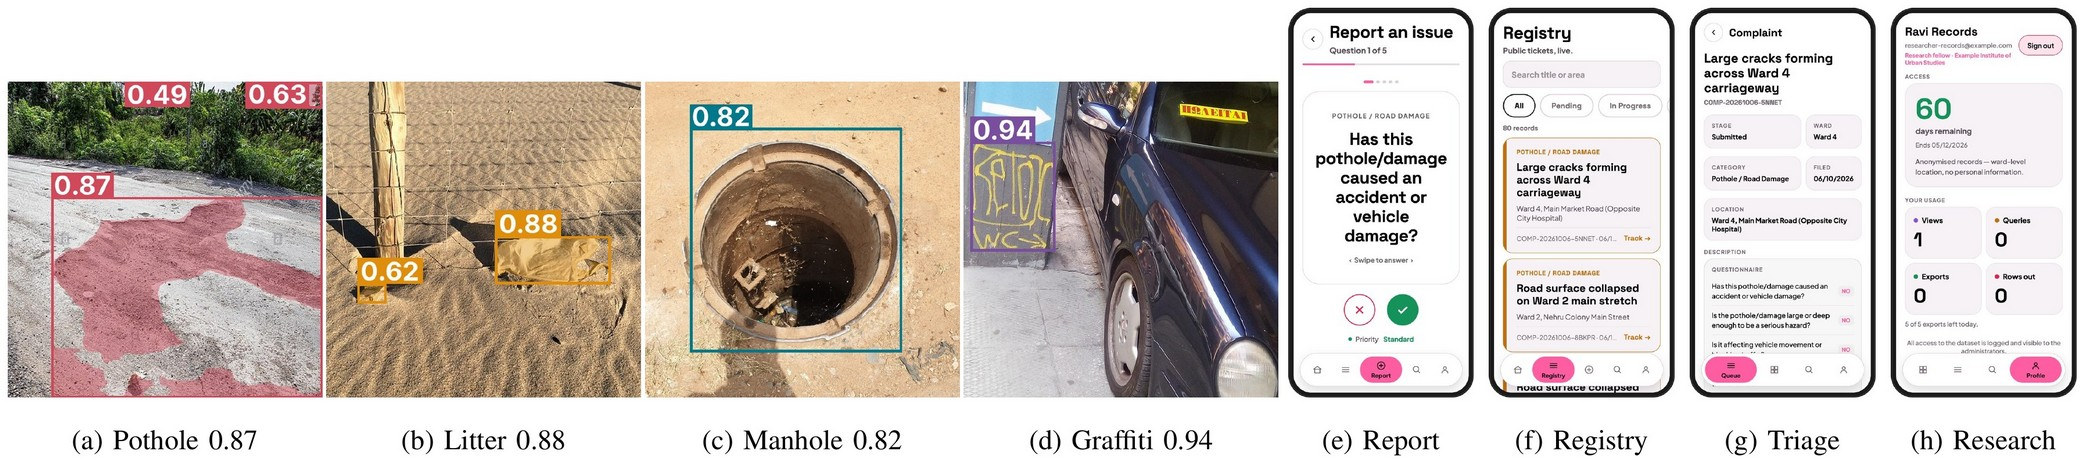
\includegraphics[width=1.00\textwidth]{figs/fig10.jpg}
\caption{(a)--(d) Stored AI evidence on validation images: predicted masks or boxes with confidence. (e)--(h) App screens: weighted swipe questionnaire with live urgency, open public registry, supervisor triage, and researcher access with expiry countdown, quota and audit notice.}
\label{fig:f10}
\end{figure*}

\begin{figure}[!t]
\centering
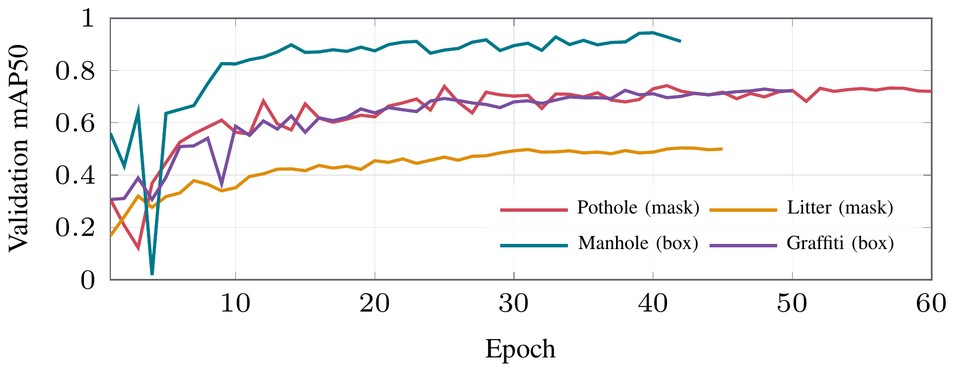
\includegraphics[width=0.95\columnwidth]{figs/fig11.jpg}
\caption{Validation mAP50 per epoch. The manhole run stopped early at epoch 42.}
\label{fig:f11}
\end{figure}

\begin{figure}[!t]
\centering
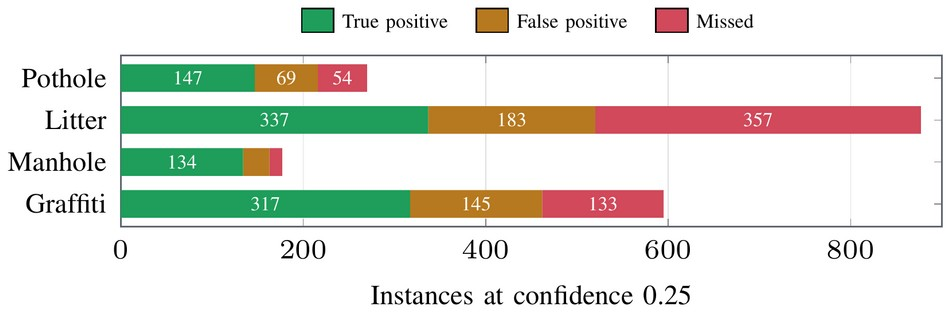
\includegraphics[width=0.95\columnwidth]{figs/fig12.jpg}
\caption{Detection outcomes on the validation sets (manhole: 134, 29, 14). Missed instances (red) are what Eq.~(\ref{eq:e5}) routes to a person.}
\label{fig:f12}
\end{figure}

\begin{figure}[!t]
\centering
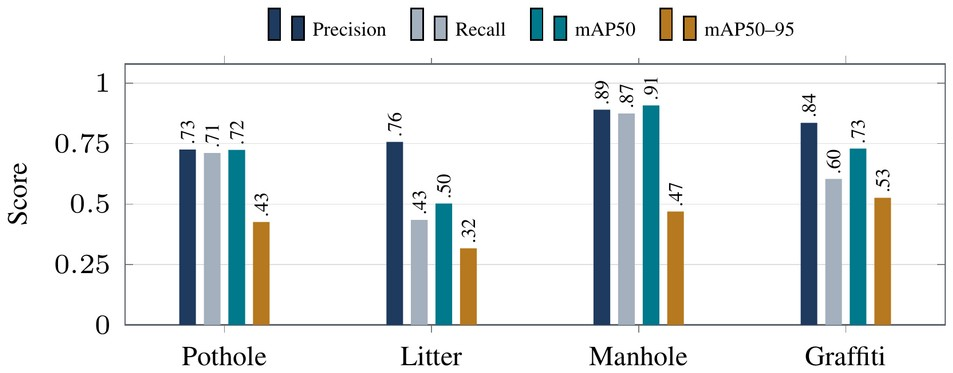
\includegraphics[width=0.95\columnwidth]{figs/fig13.jpg}
\caption{Validation metrics per model (mask metrics for the segmentation models, box metrics for the detection models).}
\label{fig:f13}
\end{figure}

\begin{figure}[!t]
\centering
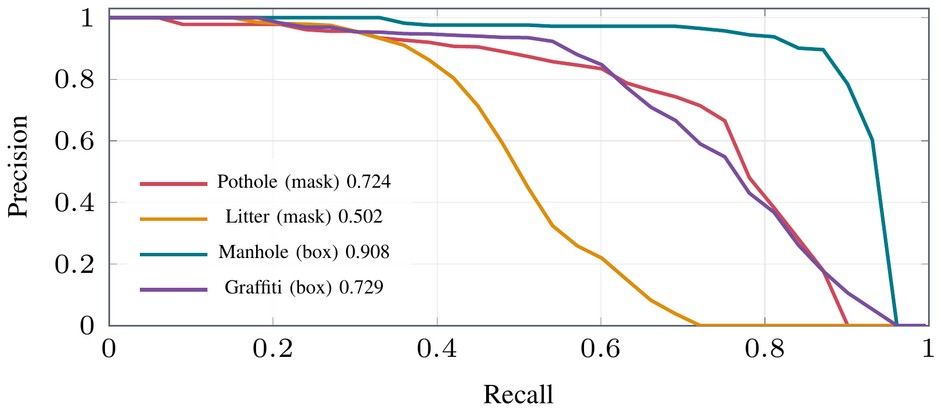
\includegraphics[width=0.94\columnwidth]{figs/fig14.jpg}
\caption{Precision--recall curves on the validation sets; legend gives AP at IoU 0.5.}
\label{fig:f14}
\end{figure}

Panels (a)--(d) of Fig.~\ref{fig:f10} are the evidence images the service stores with a complaint, drawn here on validation photos with the detection's confidence beneath each. The pothole and litter models draw masks, which the damage share $\delta$ of Eq.~(\ref{eq:e4}) needs; the manhole and graffiti models draw boxes. Panels (e)--(h) are four app screens: the citizen's questionnaire with its live urgency band, the public registry, the supervisor's triage view, and the researcher's profile with its expiry countdown and quota.

\subsection{System Validation and Demonstration Data}

All sixteen API tests passed (Fig.~\ref{fig:f15}). To exercise the dashboards we seeded 80 complaints over twelve months (Fig.~\ref{fig:f16}): 41 were accepted, 9 rejected and 19 closed, after 8.2 to 9.2 days on average.

\begin{figure}[!t]
\centering
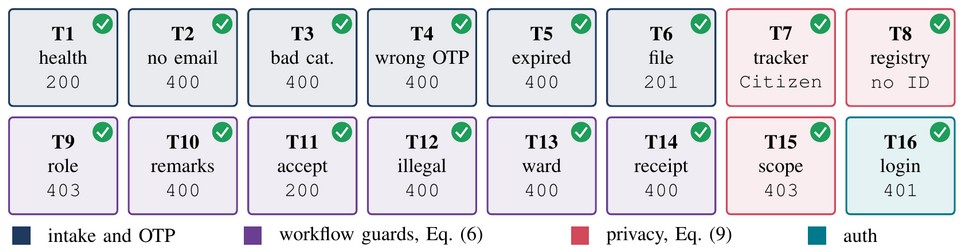
\includegraphics[width=0.96\columnwidth]{figs/fig15.jpg}
\caption{Sixteen API tests against a live server, grouped by the rule they exercise; expected and observed responses matched in all cases.}
\label{fig:f15}
\end{figure}

Fig.~\ref{fig:f15} groups the tests by the rule they check and gives the expected response in each tile. Eleven of the sixteen expect a refusal. Four cover intake: a missing email, a category outside $\mathcal{C}$, and a wrong or expired OTP. Five cover workflow guards: a field worker trying to accept (403), remarks shorter than ten characters, a rejection after acceptance, a cross-ward assignment, and a receipt requested before closure. The other two are an aggregate-only researcher asking for records (403) and a failed login (401). Each refusal comes from the server, so these rules hold whatever the client sends. Of the five tests that expect success, two check privacy: they confirm that the registry response carries no citizen identity and that the tracker shows a citizen in the history only as ``Citizen''.

Fig.~\ref{fig:f16}(a) shows how far the 80 seeded complaints progressed. Of those, 41 were accepted and 9 rejected, leaving 30 awaiting a supervisor's decision. Of the accepted complaints, 33 were assigned and 19 were closed with proof. Each stage holds fewer complaints than the one before because the workflow never skips a stage. Panel (b) shows mean days to closure between 8.2 and 9.2 for every category. With only two to nine closed complaints per category the differences are too small to interpret, and since the data is seeded, the panel shows only that the dashboards can compute the measure.

\begin{figure}[!t]
\centering
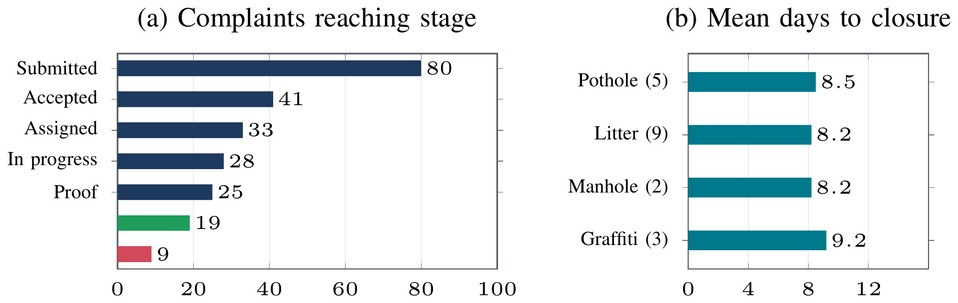
\includegraphics[width=0.96\columnwidth]{figs/fig16.jpg}
\caption{Workflow on the seeded demonstration dataset (n = 80); closed complaints per category in brackets. They exercise the dashboards only; no real ward was measured.}
\label{fig:f16}
\end{figure}

\subsection{Limitations}

Common complaints such as water leakage are unsupported for lack of data, and the models have not been tested on Indian street photos. We set the questionnaire weights and $\theta_\delta$ by hand. There is no GPS or duplicate detection, and the workflow numbers come from seeded data.

\section{Conclusion and Future Work}\label{sec:conc}

UrbanFix takes a civic complaint from the citizen's photo to a recorded repair using open-source software and public data. A per-category model checks the photo, a supervisor sets the priority, and the server enforces each step before the record is published without personal data. Next we will fine-tune on local images, fit the weights to closed complaints, add GPS and duplicate detection, and run a ward-level pilot with a municipal corporation.

\begin{thebibliography}{00}
\bibitem{b1} Ministry of Road Transport and Highways, Government of India, ``Road Accidents in India,'' annual reports 2018--2022, New Delhi.
\bibitem{b2} Ministry of Road Transport and Highways, written reply on pothole-related road accidents 2020--2024, Lok Sabha, Feb. 2026.
\bibitem{b3} Press Information Bureau, ``Grievance cell,'' Ministry of Personnel, Public Grievances and Pensions, Mar. 16, 2022. [Online]. Available: \url{https://pib.gov.in/PressReleasePage.aspx?PRID=1806610}
\bibitem{b4} Press Information Bureau, ``Disposal rate of grievance redressal mechanism,'' Apr. 2, 2025. [Online]. Available: \url{https://pib.gov.in/PressReleasePage.aspx?PRID=2117810}
\bibitem{b5} Press Information Bureau, ``CPGRAMS portal,'' Feb. 5, 2026. [Online]. Available: \url{https://pib.gov.in/PressReleasePage.aspx?PRID=2223804}
\bibitem{b6} S. K. Kanagapriya and V. Kesika, ``AI-driven anonymous civic intelligence for transparent and efficient municipal governance,'' in \textit{Proc. 7th Int. Conf. Intelligent Communication Technologies and Virtual Mobile Networks (ICICV)}, 2026, pp. 1582--1589, doi: 10.1109/ICICV68925.2026.11554648.
\bibitem{b7} R. Praveen Kumar, P. Sam Benny, Ch. Manideep, G. Sushmitha, and Md. Athfaan, ``Smart City Concern: An AI-driven multimodal civic grievance management system,'' in \textit{Proc. 6th Int. Conf. Trends in Material Science and Inventive Materials (ICTMIM)}, 2026, pp. 1894--1901, doi: 10.1109/ICTMIM68190.2026.11507401.
\bibitem{b8} P. Cholke, A. S. Mishra, V. N. Mehar, M. Chikhale, H. Marathe, and D. Nhalade, ``AI-driven complaint management system: An automated framework for prioritizing, tracking, and resolving public service complaints efficiently,'' in \textit{Proc. Int. Conf. Emerging Smart Computing and Informatics (ESCI)}, 2026, doi: 10.1109/ESCI68015.2026.11493166.
\bibitem{b9} M. Vishwanath, A. M. Vasudha, P. U. Kulkarni, M. K. Prakruthi, and V. V. Murthy, ``AI-driven smart waste management with geofencing and civic accountability,'' in \textit{Proc. 3rd Int. Conf. Emerging Applications of Material Science and Technology (ICEAMST)}, 2025, doi: 10.1109/ICEAMST67459.2025.11336075.
\bibitem{b10} S. Salunkhe, T. Salunke, A. Saware, A. Salvi, A. Patil, and R. Jolhe, ``CivicMate: An AI-driven city grievances,'' in \textit{Proc. 6th Biennial Int. Conf. Nascent Technologies in Engineering (ICNTE)}, 2026, doi: 10.1109/ICNTE66387.2026.11437408.
\bibitem{b11} G. Jocher, A. Chaurasia, and J. Qiu, ``Ultralytics YOLOv8,'' version 8.0.0, 2023. [Online]. Available: \url{https://github.com/ultralytics/ultralytics}
\bibitem{b12} B. Y. Clark, J. L. Brudney, and S.-G. Jang, ``Coproduction of government services and the new information technology: Investigating the distributional biases,'' \textit{Public Admin. Rev.}, vol. 73, no. 5, pp. 687--701, 2013, doi: 10.1111/puar.12092.
\bibitem{b13} B. Pak, A. Chua, and A. Vande Moere, ``FixMyStreet Brussels: Socio-demographic inequality in crowdsourced civic participation,'' \textit{J. Urban Technol.}, vol. 24, no. 2, pp. 65--87, 2017, doi: 10.1080/10630732.2016.1270047.
\bibitem{b14} C. E. Kontokosta and B. Hong, ``Bias in smart city governance: How socio-spatial disparities in 311 complaint behavior impact the fairness of data-driven decisions,'' \textit{Sustain. Cities Soc.}, vol. 64, Art. no. 102503, 2021, doi: 10.1016/j.scs.2020.102503.
\bibitem{b15} D. Arya, H. Maeda, S. K. Ghosh, D. Toshniwal, and Y. Sekimoto, ``RDD2022: A multi-national image dataset for automatic road damage detection,'' arXiv:2209.08538, 2022.
\bibitem{b16} Roboflow Universe, ``Pothole segmentation YOLOv8 dataset, v1,'' CC BY 4.0. [Online]. Available: \url{https://universe.roboflow.com/farzad/pothole_segmentation_yolov8}
\bibitem{b17} P. F. Proença and P. Simões, ``TACO: Trash annotations in context for litter detection,'' arXiv:2003.06975, 2020.
\bibitem{b18} sabidrahman, ``potholes, cracks and openmanholes (Road Hazards),'' Kaggle dataset. [Online]. Available: \url{https://www.kaggle.com/datasets/sabidrahman/pothole-cracks-and-openmanhole}
\bibitem{b19} C. Patrikakis, P. Kasnesis, L. Toumanidis, and A. Tzitamidis, ``STORM graffiti/tagging detection dataset,'' Univ. of West Attica, Zenodo, 2019, doi: 10.5281/zenodo.3238357.
\bibitem{b20} S. Chen, Y. Zhang, B. Song, X. Du, and M. Guizani, ``An intelligent government complaint prediction approach,'' \textit{Big Data Res.}, vol. 30, Art. no. 100336, 2022, doi: 10.1016/j.bdr.2022.100336.
\bibitem{b21} P. M. Javali, K. Naregal, A. Gudnavar, S. Athanikar, and S. Shinde, ``A web-based public grievance redressal system with image and geolocation support,'' in \textit{Proc. Int. Conf. Smart \& Sustainable Technology (INCSST)}, 2025, doi: 10.1109/INCSST64791.2025.11210297.
\bibitem{b22} S. N. Katkar, V. Makadiya, A. Mane, V. Parab, and M. Pingale, ``CivicX: An AI-driven data-centric platform for urban grievance management and intelligent plan approval,'' in \textit{Proc. Int. Conf. Communication, Computing and Emerging Technologies (IC3ET)}, 2026, pp. 631--641, doi: 10.1109/IC3ET64989.2026.11467223.
\bibitem{b23} S. F. King and P. Brown, ``Fix my street or else: Using the internet to voice local public service concerns,'' in \textit{Proc. 1st Int. Conf. Theory and Practice of Electronic Governance (ICEGOV)}, 2007, pp. 72--80, doi: 10.1145/1328057.1328076.
\bibitem{b24} M. F. Goodchild, ``Citizens as sensors: The world of volunteered geography,'' \textit{GeoJournal}, vol. 69, no. 4, pp. 211--221, 2007, doi: 10.1007/s10708-007-9111-y.
\bibitem{b25} S. L. Minkoff, ``NYC 311: A tract-level analysis of citizen--government contacting in New York City,'' \textit{Urban Affairs Rev.}, vol. 52, no. 2, pp. 211--246, 2016, doi: 10.1177/1078087415577796.
\bibitem{b26} L. Wang, C. Qian, P. Kats, C. Kontokosta, and S. Sobolevsky, ``Structure of 311 service requests as a signature of urban location,'' \textit{PLoS ONE}, vol. 12, no. 10, Art. no. e0186314, 2017, doi: 10.1371/journal.pone.0186314.
\bibitem{b27} J. Redmon, S. Divvala, R. Girshick, and A. Farhadi, ``You only look once: Unified, real-time object detection,'' in \textit{Proc. IEEE Conf. Computer Vision and Pattern Recognition (CVPR)}, 2016, pp. 779--788, doi: 10.1109/CVPR.2016.91.
\bibitem{b28} H. Maeda, Y. Sekimoto, T. Seto, T. Kashiyama, and H. Omata, ``Road damage detection and classification using deep neural networks with smartphone images,'' \textit{Comput.-Aided Civ. Infrastruct. Eng.}, vol. 33, no. 12, pp. 1127--1141, 2018, doi: 10.1111/mice.12387.
\bibitem{b29} A. Dhiman and R. Klette, ``Pothole detection using computer vision and learning,'' \textit{IEEE Trans. Intell. Transp. Syst.}, vol. 21, no. 8, pp. 3536--3550, 2020, doi: 10.1109/TITS.2019.2931297.
\bibitem{b30} R. Fan, U. Ozgunalp, B. Hosking, M. Liu, and I. Pitas, ``Pothole detection based on disparity transformation and road surface modeling,'' \textit{IEEE Trans. Image Process.}, vol. 29, pp. 897--908, 2020, doi: 10.1109/TIP.2019.2933750.
\bibitem{b31} D. Arya, H. Maeda, S. K. Ghosh, D. Toshniwal, A. Mráz, T. Kashiyama, and Y. Sekimoto, ``Deep learning-based road damage detection and classification for multiple countries,'' \textit{Autom. Constr.}, vol. 132, Art. no. 103935, 2021, doi: 10.1016/j.autcon.2021.103935.
\bibitem{b32} M. Córdova, A. Pinto, C. C. Hellevik, S. A.-A. Alaliyat, I. A. Hameed, H. Pedrini, and R. da S. Torres, ``Litter detection with deep learning: A comparative study,'' \textit{Sensors}, vol. 22, no. 2, Art. no. 548, 2022, doi: 10.3390/s22020548.
\bibitem{b33} J. Fogaça, T. Brandão, and J. C. Ferreira, ``Deep learning-based graffiti detection: A study using images from the streets of Lisbon,'' \textit{Appl. Sci.}, vol. 13, no. 4, Art. no. 2249, 2023, doi: 10.3390/app13042249.
\bibitem{b34} M. Janssen, Y. Charalabidis, and A. Zuiderwijk, ``Benefits, adoption barriers and myths of open data and open government,'' \textit{Inf. Syst. Manage.}, vol. 29, no. 4, pp. 258--268, 2012, doi: 10.1080/10580530.2012.716740.
\bibitem{b35} Y. Zheng, L. Capra, O. Wolfson, and H. Yang, ``Urban computing: Concepts, methodologies, and applications,'' \textit{ACM Trans. Intell. Syst. Technol.}, vol. 5, no. 3, pp. 1--55, 2014, doi: 10.1145/2629592.
\bibitem{b36} B. W. Wirtz, J. C. Weyerer, and C. Geyer, ``Artificial intelligence and the public sector: Applications and challenges,'' \textit{Int. J. Public Admin.}, vol. 42, no. 7, pp. 596--615, 2019, doi: 10.1080/01900692.2018.1498103.
\bibitem{b37} L. Sweeney, ``\textit{k}-anonymity: A model for protecting privacy,'' \textit{Int. J. Uncertainty, Fuzziness Knowl.-Based Syst.}, vol. 10, no. 5, pp. 557--570, 2002, doi: 10.1142/S0218488502001648.
\bibitem{b38} S. Amershi \textit{et al.}, ``Guidelines for human-AI interaction,'' in \textit{Proc. CHI Conf. Human Factors in Computing Systems}, 2019, pp. 1--13, doi: 10.1145/3290605.3300233.
\bibitem{b39} X. Wu, L. Xiao, Y. Sun, J. Zhang, T. Ma, and L. He, ``A survey of human-in-the-loop for machine learning,'' \textit{Future Gener. Comput. Syst.}, vol. 135, pp. 364--381, 2022, doi: 10.1016/j.future.2022.05.014.
\end{thebibliography}

\begin{IEEEbiography}[{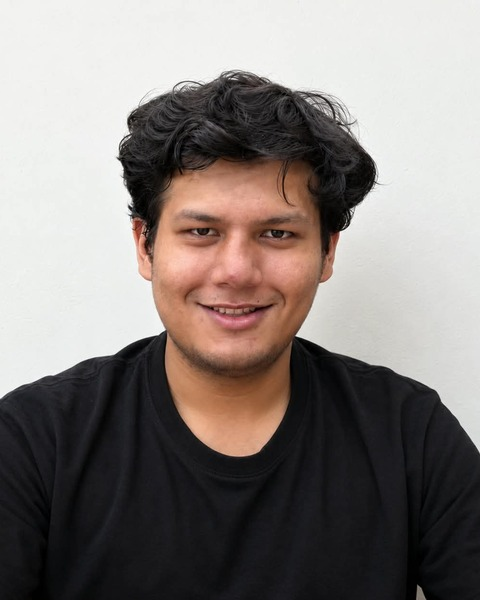
\includegraphics[width=1in,height=1.25in,clip,keepaspectratio]{photos/pancholi.jpg}}]{Parth Pancholi}
is currently pursuing the B.Tech. degree in computer science and engineering with the School of Computing Science and Engineering (SCOPE), VIT Bhopal University, Bhopal, India. He developed the UrbanFix platform presented in this article, including the YOLOv8-based photo validation models, the server-enforced complaint workflow, the public accountability registry, and the research data gateway. His research interests include computer vision, object detection, human-in-the-loop artificial intelligence, civic technology, e-governance, and privacy-preserving data sharing.
\end{IEEEbiography}

\begin{IEEEbiography}[{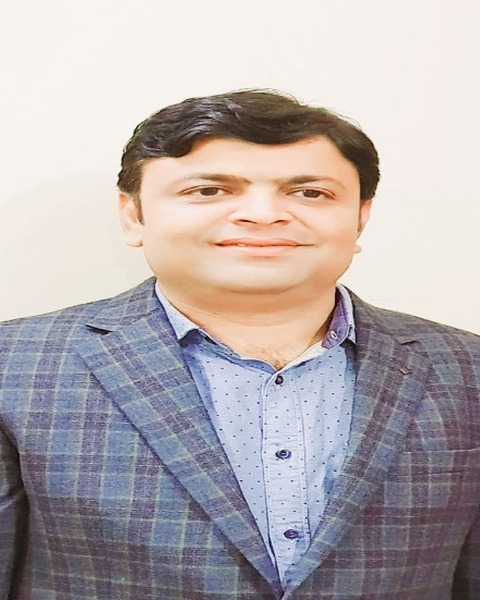
\includegraphics[width=1in,height=1.25in,clip,keepaspectratio]{photos/soni.jpg}}]{Gaurav Soni}
(Senior Member, IEEE) is a Senior Assistant Professor with the School of Computing Science and Engineering (SCOPE), VIT Bhopal University, Bhopal, India. He has 15 years of academic experience. He has published 46 articles in peer-reviewed international and national journals with high impact factors, as well as papers at international conferences held in India and abroad, and he has published six technical patents. His research interests include wireless networks, the Internet of Things (IoT), artificial intelligence, network security, flying ad hoc networks (FANETs), and vehicular ad hoc networks (VANETs).

Dr. Soni is a member of the ACM and holds an associate-level AWS certification.
\end{IEEEbiography}

\begin{IEEEbiography}[{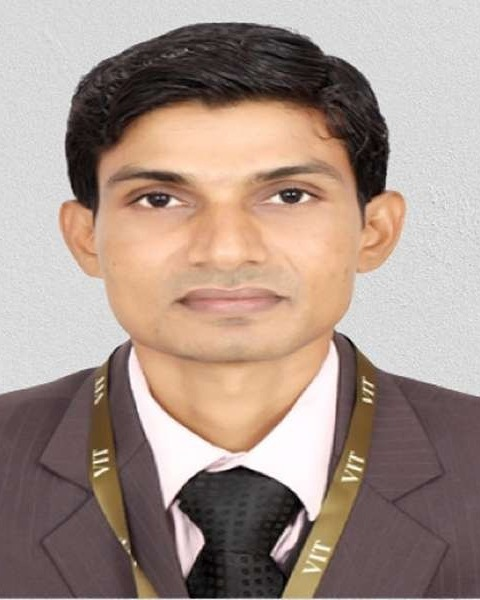
\includegraphics[width=1in,height=1.25in,clip,keepaspectratio]{photos/chandravanshi.jpg}}]{Kamlesh Chandravanshi}
received the M.Tech. and Ph.D. degrees in computer science and engineering. He is currently with the School of Computing Science and Engineering (SCOPE), VIT Bhopal University, Bhopal, India, and has 17 years of academic experience. He has 45 publications in peer-reviewed international and national journals with high impact factors and eight publications at international conferences held in India and abroad. His research interests include mobile ad hoc networks, wireless sensor networks, and the Internet of Things (IoT).

Dr. Chandravanshi serves as a reviewer for several international journals and is a Professional Member of the IACSIT.
\end{IEEEbiography}

\begin{IEEEbiography}[{
\includegraphics[width=1in,height=1.25in,clip,keepaspectratio]{photos/sahare.jpg}}]{Mahendra Sahare}
received the M.Tech. degree in computer science and engineering from RGPV, Bhopal, India, and the Ph.D. degree in computer science and engineering from RNTU, Bhopal. He is currently an Assistant Professor (Senior Grade 1) with the School of Computer Science and Engineering (SCOPE), VIT-AP University, Amaravati, India. He has more than 16 years of academic experience and has served as a Department Head and as the NBA and NAAC Criterion III Coordinator at previous institutions.

He holds three patents, has 12 publications in peer-reviewed international and national journals with high impact factors and six publications at international conferences held in India and abroad, and has published a book on artificial intelligence with Technical Press.

Dr. Sahare is a life member of ARESS and was a member of the ACM Student Chapter and the IIC at his previous institution. He received the Best Faculty Award from the management of NIIST Bhopal.
\end{IEEEbiography}

\begin{IEEEbiography}[{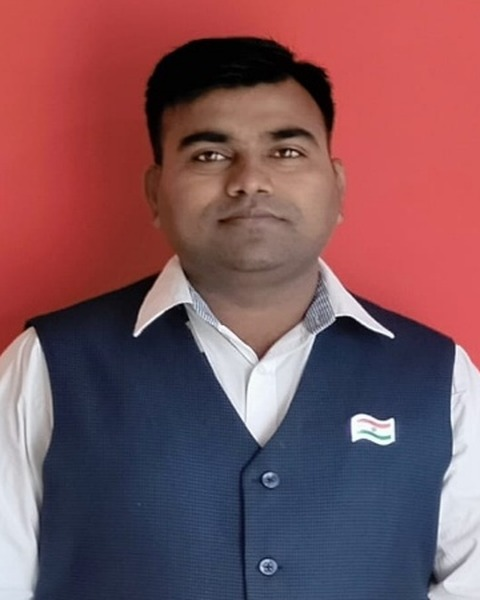
\includegraphics[width=1in,height=1.25in,clip,keepaspectratio]{photos/maurya.jpg}}]{Jay Prakash Maurya}
is currently pursuing the Ph.D. degree with SATI (Autonomous), RGPV, Bhopal, India. He received a postgraduate diploma in system database administration from CDAC, Noida, India. He is currently an Assistant Professor with the School of Computing Science and Engineering (SCOPE), VIT Bhopal University, Bhopal, India, and has 11 years of teaching and research experience. He has published more than 40 research papers in reputed international and national journals and conference proceedings, including Scopus-indexed and UGC-listed venues, and five book chapters in the fields of data mining, image processing, and network security. He also holds three patents and two copyrights. His current research interests include data mining, machine learning, soft computing, and the IoT.

Mr. Maurya is certified in CCNA, CompTIA, and system database administration by CDAC, Noida. He has conducted workshops in collaboration with IIT Bombay for the ``Smart Classroom'' and ``Bodhi Tree'' projects under the Spoken Tutorial initiative.
\end{IEEEbiography}

\EOD

\end{document}
